We describe the choices we did about representation of the data and communication between modules.
These choices are described precisely in the documentation\footnote{\url{https://github.com/ProjetPP/Documentation/}} of the project.

\section{Data model}
\label{rdf}

First, we present the data model. Its aim is to represent in a well formatted structure all data submitted to or generated by the modules. It must be able to contain raw data (as the input sentence or an output description) as well as structured data (as a parsed question). We will describe the abstract structure without detail of implementation and justify this choice.

\subsection{Abstract structure}

The data model is very close to the first order logic. The structure is defined by induction.

The grammar of this structure is given in figure \ref{datamodel:grammar}.

\begin{figure}[ht!]
$$
\begin{aligned}
S &:= \texttt{Resource list}\\
  &\mid \triple(S_1,S_2,S_3)\\
  &\mid \triple(?,S_1,S_2) \mid \triple(S_1,?,S_2) \mid \triple(S_1,S_2,?)\\
  &\mid S_1 \wedge S_2 \mid S_1 \vee S_2 \mid \neg S\\
  &\mid S_1 \cap S_2 \mid S_1 \cup S_2 \mid S_1 \setminus S_2\\
  &\mid \texttt{Sort}(S,Resource)\\
  &\mid \texttt{First}(S) \mid \texttt{Last}(S)\\
\end{aligned}
$$
\caption{Grammar of the datamodel}
\label{datamodel:grammar}
\end{figure}

A basic element is called \textsl{\bf resource}. A \textsl{resource} may represent anything in the world, a string, an integer, coordinates, a function, etc.

A \textsl{\bf list} is a finite ordered sequence of \textsl{resources}. We identify the \textsl{list} \textsl{[a]} containing only one element and the resource \textsl{a}. The use of this identification will be explained later. Moreover, a \textsl{list} must have no duplicates. For instance \textsl{[a,a]} is not a list and need to be simplified as \textsl{[a]}. We can see \textsl{lists} as finite totally ordered set.

The other atomic elements are the boolean values \textsl{\bf true} and \textsl{\bf false}. They are not \textsl{resources} as previously defined. Nevertheless, we admit \textsl{resources} "true" and "false" but we cannot apply logic operation on them.

A \textsl{\bf triple} is a 3-tuple containing in this order:
\begin{itemize}
    \item a subject: what the triple refers to,
    \item a predicate: the relation between the subject and the object,
    \item an object: what the property of the subject refers to.
\end{itemize}

For instance, we can represent the sentence "Isaac \textsc{Newton} was born on the 25 December 1642 (Julian)" by the triple
\begin{figure}[!ht]
    \centering
    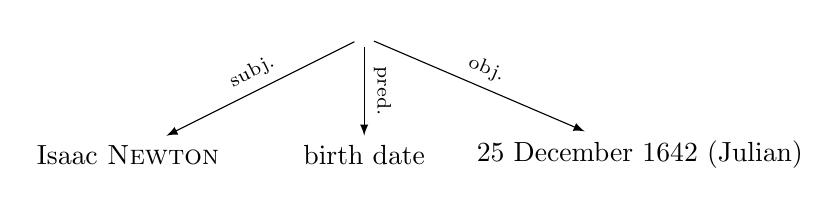
\begin{tikzpicture}
        \node (1) at (7,7) {$\triple$};
        \node (11) at (4,5.5) {Isaac \textsc{Newton}};
        \node (12) at (7,5.5) {birth date};
        \node (13) at (10.5,5.5) {25 December 1642 (Julian)};
        \draw[->, >=latex] (1) edge node[sloped, anchor=center, above] {\scriptsize{subj.}} (11);
        \draw[->, >=latex] (1) edge node[sloped, anchor=center, above] {\scriptsize{pred.}} (12);
        \draw[->, >=latex] (1) edge node[sloped, anchor=center, above] {\scriptsize{obj.}} (13);
    \end{tikzpicture}
\end{figure}
\FloatBarrier
In other terms, we can consider than the description of Isaac \textsc{Newton} has an entry "birth date" whose value is "25 December 1642 (Julian)" or any equivalent value.

It is reasonable to associate to each triple a boolean value depending upon whether the triple is true or not. Generally triples contains \textsl{lists} with more than one value. So we define the node \textsl{full triple} 
\begin{center}
\textsl{full triple: list$^3\rightarrow$ bool}
\end{center}
and we define its value as $$(a,b,c)=\bigwedge_{i=1}^{n_a}\bigwedge_{j=1}^{n_b}\bigwedge_{k=1}^{n_c} (\textsl{a}_i,\textsl{b}_j,\textsl{c}_k)$$where $a=[a_1,\ldots,a_{n_a}]$, $b=[b_1,\ldots,b_{n_b}]$ and $c=[c_1,\ldots,c_{n_c}]$.

This structure is needed to check if a statement is true. That naturally correspond to yes/no questions.

A kind of natural yes/no question which are not handled by \textsl{full triple} are existential questions: "Is there a... ?". To represent them, we use a node \textsl{\bf exists} (also denoted by $\exists$)
\begin{center}
\textsl{exists: list$\rightarrow$ bool}
\end{center}
and the evaluations is \textsl{exists$(l) = \begin{cases}
\textsl{true} & \text{if }l\neq\emptyset\\
\textsl{false} & \text{if }l=\emptyset
\end{cases}$}. This node checks whether the list is non empty.

The usual boolean operations: and ($\wedge$), or ($\vee$), not ($\neg$).

\bigskip

The usual operations on lists: union, intersection, difference. They do not keep the order of the \textsl{lists}.

We also allow \textsl{incomplete triples}. An incomplete triple is a triple with a "hole": we know only two values and we want the list of all values which satisfy the triple. There is 3 type of required triples: for subject, predicate and object. They have the type
\begin{center}
\textsl{incomplete triple: list$^2\rightarrow$ list}
\end{center}
and the evaluations are
\begin{itemize}
    \item for subject: $\textsl{incomplete triple}_{\textsl{subject}}(a,b) = \textsl{list}(\{\textsl{x}\mid(x,a,b)\})$ denoted by $(?,a,b)$,
    \item for predicate: $\textsl{incomplete triple}_{\textsl{predicate}}(a,b) = \textsl{list}(\{\textsl{x}\mid(a,x,b)\})$ denoted by $(a,?,b)$,
    \item for object: $\textsl{incomplete triple}_{\textsl{object}}(a,b) = \textsl{list}(\{\textsl{x}\mid(a,b,x)\})$ denoted by $(a,b,?)$.
\end{itemize}

We define two additional nodes: \textsl{sort}, \textsl{first} and \textsl{last}.

\begin{center}
\textsl{sort: list$\times$resource$\rightarrow$list}
\end{center}
This function \textsl{sort} take a list and a predicate and sort the element of the list in the increasing order according to the value returned by the predicate. More formally, let $l=[l_1,\ldots,l_n]$, $p$ a predicate and $a_i$ such that $\forall i\in\llbracket1,n\rrbracket, (l_i,p,a_i)$. Then, \textsl{sort}$(l,p) = [l_{\sigma(1)},\ldots,l_{\sigma(n)}]$ where $\sigma\in\mathfrak{S}_n$ and $\forall (i,j)\in\llbracket 1,n\rrbracket^2, \sigma(i)<\sigma(j) \Leftrightarrow a_i \leqslant a_j$. This definition assume that the predicate $p$ associate to the list a totally ordered set.

The function \textsl{first} returns the first (smallest if the list is ordered) element of a list.

\begin{center}
\textsl{first: list$\rightarrow$ resource}
\end{center}

The function \textsl{last} returns the last (greatest if the list is ordered) element of a list.

\begin{center}
\textsl{last: list$\rightarrow$ resource}
\end{center}

These nodes are useful when a triple can return a list with more than one element and we need only one. The difficulty is to find what is the correct order to choose.

\bigskip

A tree which represents a sentence is called a 
{\bf normal form} of this sentence. There may be several normal forms for a sentence. Indeed, the trees $(a,b,c\cap d)$ and $(a,b,c)\wedge(a,b,d)$ have the same meaning.\todo{NO}

\subsection{Examples}

To clarify the previous definitions, we give some examples. We give some question followed by their normal form.

\FloatBarrier
\bigskip

"Was Isaac \textsc{Newton} born on the 25 December 1642 (Julian)?"

\begin{figure}[!ht]
    \centering
    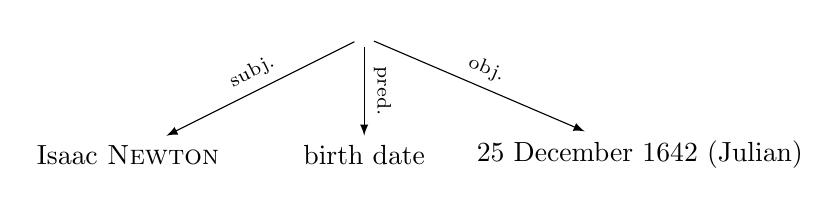
\begin{tikzpicture}
        \node (1) at (7,7) {$\triple$};
        \node (11) at (4,5.5) {Isaac \textsc{Newton}};
        \node (12) at (7,5.5) {birth date};
        \node (13) at (10.5,5.5) {25 December 1642 (Julian)};
        \draw[->, >=latex] (1) edge node[sloped, anchor=center, above] {\scriptsize{subj.}} (11);
        \draw[->, >=latex] (1) edge node[sloped, anchor=center, above] {\scriptsize{pred.}} (12);
        \draw[->, >=latex] (1) edge node[sloped, anchor=center, above] {\scriptsize{obj.}} (13);
    \end{tikzpicture}
\end{figure}

\FloatBarrier
\bigskip

"Is Brussels the capital of Belgium and the European Union?"

\begin{figure}[!ht]
    \centering
    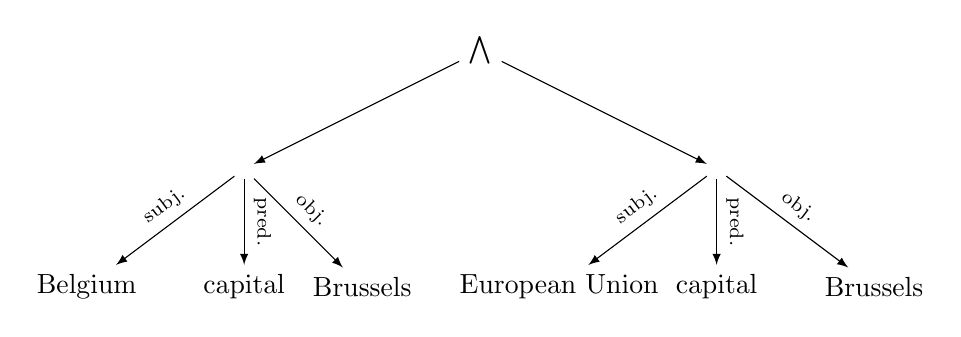
\begin{tikzpicture}
        \node (0) at (10,8.5) {$\bigwedge$};
        \node (1) at (7,7) {$\triple$};
        \node (11) at (5,5.5) {Belgium};
        \node (12) at (7,5.5) {capital};
        \node (13) at (8.5,5.5) {Brussels};
              
        \node (2) at (13,7) {$\triple$};
        \node (21) at (11,5.5) {European Union};
        \node (22) at (13,5.5) {capital};
        \node (23) at (15,5.5) {Brussels};

        \draw[->, >=latex] (0) edge node[sloped, anchor=center, above] {} (1);
        \draw[->, >=latex] (1) edge node[sloped, anchor=center, above] {\scriptsize{subj.}} (11);
        \draw[->, >=latex] (1) edge node[sloped, anchor=center, above] {\scriptsize{pred.}} (12);
        \draw[->, >=latex] (1) edge node[sloped, anchor=center, above] {\scriptsize{obj.}} (13);
        \draw[->, >=latex] (0) edge node[sloped, anchor=center, above] {} (2);
        \draw[->, >=latex] (2) edge node[sloped, anchor=center, above] {\scriptsize{subj.}} (21);
        \draw[->, >=latex] (2) edge node[sloped, anchor=center, above] {\scriptsize{pred.}} (22);
        \draw[->, >=latex] (2) edge node[sloped, anchor=center, above] {\scriptsize{obj.}} (23);
    \end{tikzpicture}
\end{figure}
            
\FloatBarrier
\bigskip

"Who were the presidents of the United States?"
\begin{figure}[!ht]
    \centering
    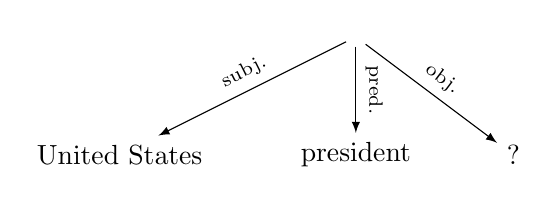
\begin{tikzpicture}
        \node (3) at (8,8.5) {$\triple$};
        \node (4) at (8,7) {president};
        \node (5) at (5,7) {United States};
        \node (6) at (10,7) {?};

        \draw[->, >=latex] (3) edge node[sloped, anchor=center, above] {\scriptsize{subj.}} (5);
        \draw[->, >=latex] (3) edge node[sloped, anchor=center, above] {\scriptsize{obj.}} (6);
        \draw[->, >=latex] (3) edge node[sloped, anchor=center, above] {\scriptsize{pred.}} (4);
    \end{tikzpicture}
\end{figure}

\FloatBarrier
\bigskip

"Who is mayor of the capital of Kreis Bergstraße?"
\begin{figure}[!ht]
    \centering
    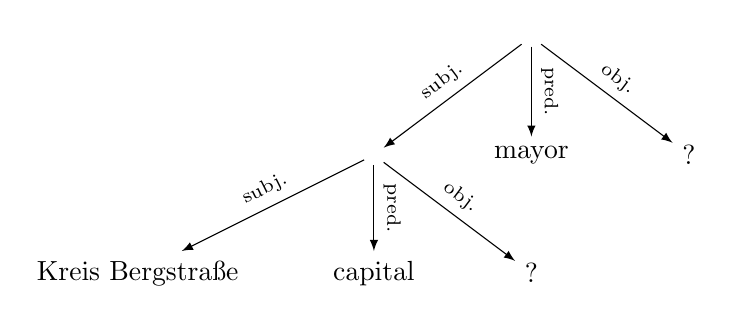
\begin{tikzpicture}
        \node (0) at (10,10) {$\triple$};
        \node (1) at (10,8.5) {mayor};
        \node (2) at (12,8.5) {?};
        \node (3) at (8,8.5) {$\triple$};
        \node (4) at (8,7) {capital};
        \node (5) at (5,7) {Kreis Bergstraße};
        \node (6) at (10,7) {?};

        \draw[->, >=latex] (0) edge node[sloped, anchor=center, above] {\scriptsize{obj.}} (2);
        \draw[->, >=latex] (0) edge node[sloped, anchor=center, above] {\scriptsize{pred.}} (1);
        \draw[->, >=latex] (0) edge node[sloped, anchor=center, above] {\scriptsize{subj.}} (3);
        \draw[->, >=latex] (3) edge node[sloped, anchor=center, above] {\scriptsize{subj.}} (5);
        \draw[->, >=latex] (3) edge node[sloped, anchor=center, above] {\scriptsize{obj.}} (6);
        \draw[->, >=latex] (3) edge node[sloped, anchor=center, above] {\scriptsize{pred.}} (4);
    \end{tikzpicture}
\end{figure}

\FloatBarrier
\bigskip

"What is the birth date of the first president of Germany?"
\begin{figure}[!ht]
    \centering
    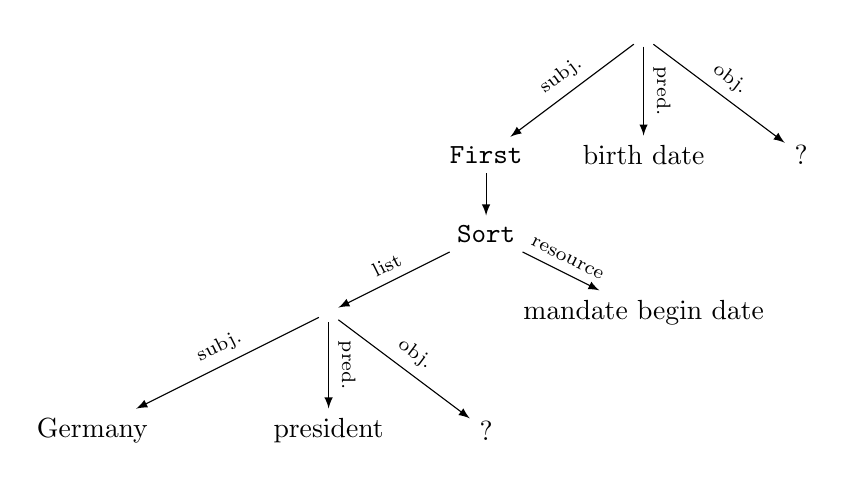
\begin{tikzpicture}
        \node (0) at (10,10) {$\triple$};
        \node (1) at (10,8.5) {birth date};
        \node (2) at (12,8.5) {?};
        \node (8) at (8,8.5) {\texttt{First}};
        \node (9) at (8,7.5) {\texttt{Sort}};
        \node (10) at (10,6.5) {mandate begin date};
        \node (3) at (6,6.5) {$\triple$};
        \node (4) at (6,5) {president};
        \node (5) at (3,5) {Germany};
        \node (6) at (8,5) {?};

        \draw[->, >=latex] (0) edge node[sloped, anchor=center, above] {\scriptsize{obj.}} (2);
        \draw[->, >=latex] (0) edge node[sloped, anchor=center, above] {\scriptsize{pred.}} (1);
        \draw[->, >=latex] (0) edge node[sloped, anchor=center, above] {\scriptsize{subj.}} (8);
        \draw[->, >=latex] (8) edge node[sloped, anchor=center, above] {} (9);
        \draw[->, >=latex] (9) edge node[sloped, anchor=center, above] {\scriptsize{resource}} (10);
        \draw[->, >=latex] (9) edge node[sloped, anchor=center, above] {\scriptsize{list}} (3);
        \draw[->, >=latex] (3) edge node[sloped, anchor=center, above] {\scriptsize{subj.}} (5);
        \draw[->, >=latex] (3) edge node[sloped, anchor=center, above] {\scriptsize{obj.}} (6);
        \draw[->, >=latex] (3) edge node[sloped, anchor=center, above] {\scriptsize{pred.}} (4);
    \end{tikzpicture}
\end{figure}

\FloatBarrier
\bigskip

"Is there a medical treatment for Ebola?"
\begin{figure}[!ht]
    \centering
    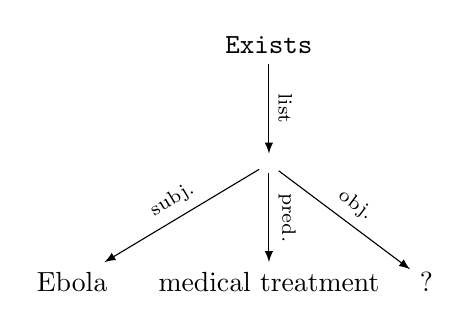
\begin{tikzpicture}
        \node (0) at (10,8.5) {\texttt{Exists}};
        \node (1) at (10,7) {$\triple$};
        \node (11) at (7.5,5.5) {Ebola};
        \node (12) at (10,5.5) {medical treatment};
        \node (13) at (12,5.5) {?};

        \draw[->, >=latex] (0) edge node[sloped, anchor=center, above] {\scriptsize{list}} (1);
        \draw[->, >=latex] (1) edge node[sloped, anchor=center, above] {\scriptsize{subj.}} (11);
        \draw[->, >=latex] (1) edge node[sloped, anchor=center, above] {\scriptsize{pred.}} (12);
        \draw[->, >=latex] (1) edge node[sloped, anchor=center, above] {\scriptsize{obj.}} (13);
    \end{tikzpicture}
\end{figure}

\FloatBarrier
\bigskip

"Who are the children of François \textsc{Mitterrand} and Anne \textsc{Pingeot}?"
\begin{figure}[!ht]
    \centering
    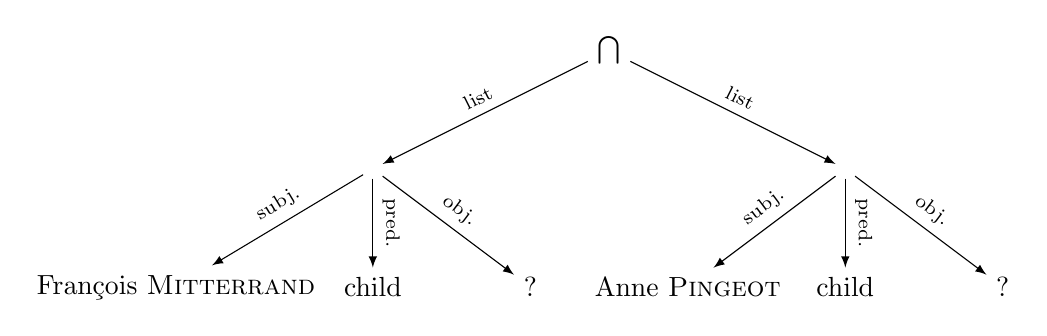
\begin{tikzpicture}
        \node (0) at (10,8.5) {$\bigcap$};
        \node (1) at (7,7) {$\triple$};
        \node (11) at (4.5,5.5) {François \textsc{Mitterrand}};
        \node (12) at (7,5.5) {child};
        \node (13) at (9,5.5) {?};
                  
        \node (2) at (13,7) {$\triple$};
        \node (21) at (11,5.5) {Anne \textsc{Pingeot}};
        \node (22) at (13,5.5) {child};
        \node (23) at (15,5.5) {?};

        \draw[->, >=latex] (0) edge node[sloped, anchor=center, above] {\scriptsize{list}} (1);
        \draw[->, >=latex] (1) edge node[sloped, anchor=center, above] {\scriptsize{subj.}} (11);
        \draw[->, >=latex] (1) edge node[sloped, anchor=center, above] {\scriptsize{pred.}} (12);
        \draw[->, >=latex] (1) edge node[sloped, anchor=center, above] {\scriptsize{obj.}} (13);
        \draw[->, >=latex] (0) edge node[sloped, anchor=center, above] {\scriptsize{list}} (2);
        \draw[->, >=latex] (2) edge node[sloped, anchor=center, above] {\scriptsize{subj.}} (21);
        \draw[->, >=latex] (2) edge node[sloped, anchor=center, above] {\scriptsize{pred.}} (22);
        \draw[->, >=latex] (2) edge node[sloped, anchor=center, above] {\scriptsize{obj.}} (23);
    \end{tikzpicture}
\end{figure}
\FloatBarrier

\subsection{Software point of view}

All normalised structures of the PPP are JSON-serializable, i.e. they are trees made of instances of the following types:
\begin{itemize}
    \item \texttt{Object}
    \item \texttt{List}
    \item \texttt{String}
    \item \texttt{Number}
    \item \texttt{Boolean}
    \item \texttt{Null}
\end{itemize}

We chose to represent all normalised data as trees. We use the previous nodes and we have a \textsl{missing} node to represent the '?' in incomplete triples.

The node \texttt{resource} to represent the previous abstract node \textsl{resource} and \textsl{bool}. Moreover, we identify the \textsl{resource} "true" and the boolean value \textsl{true} and the same for "false" and \textsl{false}. This identification is not problematic for type because we assume modules creates only well-formed expressions.

We add to the nodes we defined above some new features:
\begin{itemize}
    \item a \texttt{sentence} node: a question in natural language like "Who is George Washington?",
    \item we can precise a type to \texttt{resource} and \texttt{missing} nodes. For example, if we choose as range "time" to the missing node ? in the triple (George Washington, birth, ?) this triple with hole can only return time points.
\end{itemize}

For example, the work of the question parsing module is to transform 
\begin{verbatim}
{
    "type": "sentence", 
    "value": "Who is George Washington?"
}
\end{verbatim}
into 
\begin{verbatim}
{
    "type":
        "triple",
    "subject":{
        "type": "resource",
        "value": "George Washington"
    },
    "predicate":{
        "type": "resource",
        "value": "identity"
    },
    "object":{
        "type": "missing"
    }
}
\end{verbatim}

The basic value types are 
\begin{itemize}
    \item \texttt{string},
    \item \texttt{boolean},
    \item \texttt{time} (encoded according to ISO 8061\footnote{\url{http://www.iso.org/iso/home/standards/iso8601.htm}}),
    \item \texttt{math-latex} (for mathematical formulas written with \LaTeX),
    \item \texttt{geo-json} (for geographic data, based on GeoJson\footnote{\url{http://geojson.org/}}).
\end{itemize}

\section{Communication}

Modules communicate with the core via HTTP requests.

The core sends them a JSON object, and they return another one.

The basic idea is that the core iterates requests to modules, which return a simplified tree, until the core gets a complete response, ie. a tree without any `missing` node.

During these exchanges, we keep a trace of the different steps between the original request and the current tree. The structure of a trace is a list of such trace items:
\begin{verbatim}
{
    "module":
        "<name of the module>", 
    "tree":{
        <answer tree>
    },
    "measures":{
        "relevance": <relevance of the answer>,
        "accuracy": <accuracy of the answer>
    }
}
\end{verbatim}

The measure field contains two values: relevance and accuracy.

\begin{itemize}
    \item \texttt{accuracy} is a self-rating of how much the module may have correctly understood (ie. not misinterpreted) the request/question. It is a float between 0 and 1.
    \item \texttt{relevance} is a self-rating of how much the tree has been improved (i.e. progressed on the path of becoming a useful answer). A positive float (not necessarily greater that 1; another module might use it to provide a much better answer).
\end{itemize}

We do not provide a method to compute these values. We have to trust every modules.

This form allows each module to access to the previous results, particularly to the request of the user. The objects for request and response contain some extra data, such as the language used.

We can use these measure to chose the best answer to display it at the first position in the UI. Modules can use them too. For instance, if there are two modules for question parsing, a module will choose one of the two answers based on these marks.

The data model have been implemented in a nice set of objects in both Python\footnote{\url{http://github.com/ProjetPP/PPP-datamodel-Python/}} and PHP\footnote{\url{http://github.com/ProjetPP/PPP-datamodel-PHP/}} in order to help the writing of modules.

We could define a linear representation for the trace, using the representation of the datamodel, but it is not relevant. Indeed, this information will never be printed on the user interface.

\begin{figure}[!ht]
    \centering
    \label{datamodel:struct}
    \newlength{\moduledistance}
\setlength{\moduledistance}{1cm}
\overfullrule=2cm
\tikzset{
    module/.style={
           rectangle,
%           rounded corners,
           draw=mDarkTeal, very thick,
           minimum width=3cm,
           minimum height = 0.7cm,
           node distance = 1.5cm,
           inner sep=2pt,
           text centered,
           },
}

\tikzset{
    core/.style={
           circle,
           draw=mDarkTeal, very thick,
           minimum width=2cm,
           inner sep=2pt,
           text centered,
           },
}

\tikzset{
    arrow/.style={
           ->,
           draw=mDarkTeal, very thick,
    }
}

\tikzset{
    darrow/.style={
           <->,
           draw=mDarkTeal, very thick,
    }
}

\begin{tikzpicture}[->,>=stealth']
    \node[core] (core) {
        Core
    };
    \node[module,
          right of=core,
          right=\moduledistance,
          ] (grammatical) {
          Grammatical
    };
    \node[module,
          below of=grammatical,
          ] (standalone) {
        \begin{tabular}{c}
        Machine Learning\\Standalone
        \end{tabular}
    };
    \node[module,
          above of=grammatical,
          ] (reformulation) {
        \begin{tabular}{c}
        Machine Learning\\Reformulation
        \end{tabular}
    };
    \node[module,
          left of=core,
          left=\moduledistance,
          ] (wikidata) {
        Wikidata
    };
    \node[module,
          above of=wikidata,
          ] (cas) {
        Computer Algebra
    };
    \node[module,
          below of=wikidata,
          ] (spellchecker) {
        Spell-checker
    };
    \node[module,
          above of=core,
          above=1cm,
          ] (webui) {
        \begin{tabular}{c}
        Web User\\
        Interface
        \end{tabular}
    };
    \node[module,
          above of=reformulation,
%          right=\moduledistance,
          ] (logging) {
        Logging backend
    };
    \draw[mLightBrown,thick] ($(reformulation.north west)+(-0.3,0.3)$)  rectangle node[yshift=-2.5cm,below] {Question Parsing} ($(standalone.south east)+(0.3,-0.3)$);
    \draw[mLightBrown,thick] ($(cas.north west)+(-0.3,0.3)$)  rectangle node[yshift=-2.5cm,below] {Other modules} ($(spellchecker.south east)+(0.3,-0.3)$);

    \draw [darrow] (core)          -- node{} (cas.south east);
    \draw [darrow] (core)          -- node{} (wikidata.east);
    \draw [darrow] (core)          -- node{} (spellchecker.north east);
    \draw [darrow] (core)          -- node{} (reformulation.south west);
    \draw [darrow] (core)          -- node{} (grammatical.west);
    \draw [darrow] (core)          -- node{} (standalone.north west);
    \draw [darrow] (core)          -- node{} (webui.south);
    \draw [darrow] (webui)         -- node{} (logging.west);
    \draw [arrow]  (logging)       -- node{} (reformulation.north);
    \draw [arrow]  (grammatical)   -- node{} (reformulation.south);

\end{tikzpicture}

    \caption{Architecture of the PPP}
\end{figure}

\FloatBarrier

\section{Evolution of data model}

In the first version of the data model, there were only incomplete triples. It allowed to represent most of simple open questions like "When is Douglas Adams born?" but not composed or yes/no questions because its semantic power was intrinsically lower.
